\documentclass{article}
\usepackage[utf8]{inputenc}
\usepackage[T1]{fontenc}
\usepackage{graphicx}
\usepackage{hyperref}
\usepackage{geometry}
\geometry{margin=1in}

\title{WILLINS (D Thomas}
\date{Encyclopaedia Britannica (1771)}

\begin{document}
\maketitle

\section*{Historical source}
\textbf{Entry ID:} \texttt{entry-willins-d-thomas-258} \\
\textbf{Volume ID:} 191679021 \\
\textbf{Character Count:} 2106

\subsection*{Extracted Text}
WILLINS (D Thomas), a celebrated English Myckling, was born at Great Bodwin, in WildHere, in 1611, and fludied at Chrift-church college, Oxford. When that city was parturient for the king, the among other scholars, bore must be his Majidity, and devoted his three hours to the flyt of phyfeic. The garrior of Oxford at Leughr furnerdening to the patmanie, he applied himself to the practice of his pacification and foam rendered himself famous by his care and full. He appropriated a room as an contrary for driven revoc according to the church of England, whether end of the loyalists in Oxford only without. In 1604, he became Seeldian profiler of natural philosophy, and the fame year took the degree of dochor of phyfe. In 1604, he discovered the famonic medicinal prins at Allftrop, our Brackley. He was one of the first members of the Royal Society, and from made his name illustrious by his excellent writings. In 1605 after the first of London, he traveled to Wilminker; and his practice became greater than that of any of the physicians his contemporaries. Soon after he farfetment in London, his only for Thomas falling into a companion, the feet him to Monopolier in France for the recovery of his health; and it proved fucetful. His wife allo boating under the frame different the areas of providing for his family, died in 1670. He died at his house in So Bharti's in Oregon, and was buried near her in fifathmande abby. Dr Willis was extremely mournish and mannikians, and refrufed the honour of knightthood. He was remarkably proust. As he role early in the morning, that the maybe he pointed across foreign forces, which conclually frequested before he vifited his patients, he procured prayers to be read beyond the secundance times while he lives and at his death settled a ifgood of such pernum to continue them. He was a liberal benefactor to the poor wherever he came, having from his only practice adopted yet of his profits to charitable use. He was exact and re-gular is all his hours; a and through his table was the refert of molt of the great men of London, yet he was remarkable



\section*{Source record}
\begin{itemize}
\item \textbf{Dataset:} \texttt{NationalLibraryOfScotland/encyclopaedia\_britannica\_illustrated}
\item \textbf{Dataset Revision:} \texttt{309f765b1ecc83e0a7f7762e44b4a927a7555443}
\item \textbf{Page ID:} \texttt{britannica:309f765b1ecc83e0a7f7762e44b4a927a7555443:train:258} \\
  \textbf{Filename:} \texttt{page-0258-631a7ae7df34.jpg} \\
  \textbf{Row Index:} 258 \\
  \textbf{SHA256:} \texttt{631a7ae7df340a64...}
\end{itemize}

\begin{figure}[h]
\centering
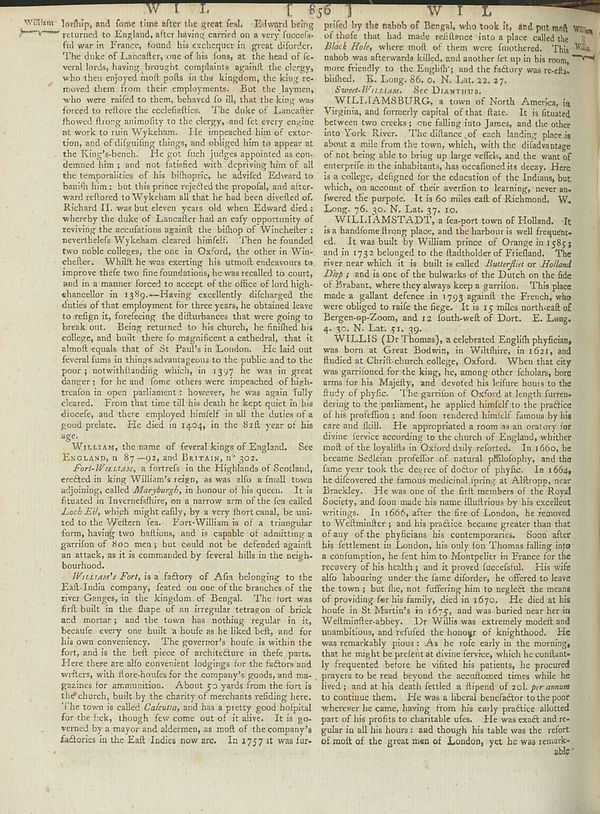
\includegraphics[width=0.85\textwidth]{../scans/page-0258-631a7ae7df34.jpg}
\caption*{Source scan: \texttt{page-0258-631a7ae7df34.jpg}}
\end{figure}

\end{document}
